\documentclass[12pt, preprint]{aastex}
\usepackage{bm}
\usepackage{amsmath}


\newcommand{\setof}[1]{\left\{{#1}\right\}}
\newcommand{\given}{\,|\,}
\newcommand{\dd}{\mathrm{d}}
\newcommand{\catalog}{\bm{Q}}
\newcommand{\pars}{\bm{\theta}}
\newcommand{\bs}[1]{\boldsymbol{#1}}

\newcommand{\Msun}{\ifmmode {M_{\odot}}\else${M_{\odot}}$\fi}

\begin{document}

\title{Modeling the X-Ray Populations of NGC 55}
\author{some combination of JJA, AZ, TF, and others}
\date{NOT READY}

\begin{abstract}
Really exciting abstract that will make everyone want to read this paper.
\end{abstract}

\section{Introduction}

{\it Chandra} has revolutionized our understanding of the X-ray emitting objects. It's unprecedented angular precision and collecting area allows it to identify dozens of resolved sources in nearby galaxies. Studies of individual objects have yielded a deeper insight into the physical processes forming the bulk of individually identified sources, low and high mass X-ray binaries (XRBs), as well as a rare, but important subset, the ultra-luminous X-ray sources (ULXs). High mass binaries, in particular, are formed from the accretion of an early-type star onto either a neutron star or black hole. Their relatively short lifetimes requires that these systems cannot travel far away from their birth site, and indeed observations show the majority of luminous X-ray sources are near star forming regions. 

NGC 55 is a relatively transparent, edge-on, nearby galaxy. Using the {\it Hubble Space Telescope}, and other optical telescopes, we have been able to identify a near-complete sample of star forming regions. For each region, multi-band photometry provides an estimate of the star formation history. 

In this work, we simulate the expected number, position, and characteristics of the X-ray binary population, given our sample of star forming regions, as well as the star formation history of the overall galaxy. We then apply a Bayesian method to generate a likelihood function comparing the resulting distribution with the observed X-ray sample.



\section{Statistical Method}

Our goal is to identify quantitatively how the individual HMXBs formed in our sample. 

We begin with Bayes' Rule:
\begin{equation}
P( M \given D ) = \frac{P( D \given M ) P(M)}{P(D)},
\end{equation}
where $M$ is the model and $D$ is the data. For any individual HMXB, the evolution can be determined uniquely (at least to first order) by its initial masses, $M_1$ and $M_2$, its initial binary separation, $a$, and the kick velocity it received after the primary collapsed to form a NS or BH, $\vec{v_k}$. Hereafter, $M$ includes both these six explicit model parameters ($M_1$, $M_2$, $a$, and $\vec{v_k}$), and our implicit model prescriptions and assumptions to follow the formation of HMXBs. For our model here, we ignore higher order effects such as differences in metallicity and the exact chemical abundance.
\begin{equation}
P ( D \given M ) = P(L_x, \vec{m}, \alpha, \delta \given M).
%P ( D \given M ) = P(L_x, \vec{m}, \alpha, \delta \given M_1, M_2, a, \vec{v_k}).
\end{equation}
We use vector notation for the magnitudes, because an individual object may have been observed using multiple filters. 
%In this case, $D$ includes the set of observed X-ray luminosities ($\bs{L_x}$), companion optical magnitudes ($\bs{\vec{m}}$), and sky positions ($\bs{\alpha}$, $\bs{\delta}$):
%\begin{equation}
%P ( D \given M ) = P( \bs{L_x}, \bs{\vec{m}}, \bs{\alpha}, \bs{\delta} \given M),
%\end{equation}
%here we use bold quantities to identify the set of individual objects. We use vector notation for the magnitudes, because an individual object may have been observed using multiple filters. The posterior probability over the entire set of observables is the product over the posterior probability over the observed quantities for each X-ray binary:
%\begin{equation}
%P( \bs{L_x}, \bs{\vec{m}}, \bs{\alpha}, \bs{\delta} \given M) = \prod_i P( L_x, \vec{m}, \alpha, \delta \given M).
%\end{equation}
We now marginalize over the companion mass ($M_2$), the systemic velocity ($v_{\rm sys}$), the birth time ($t_b$), and from which star forming region each system was formed ($C$):
\begin{equation}
P( L_x, \vec{m}, \alpha, \delta \given M) = \sum_{{\rm all}\ C} \int \int \int P( L_x, \vec{m}, \alpha, \delta, M_2, v_{\rm sys}, t_b, C \given M)\ \dd M_2\ \dd v_{\rm sys}\ \dd t_b.
\end{equation}
There are an integer number of star forming regions, so we expressed the integral over $C$ as a sum over the known set of star forming regions. This assumes a complete census of the star forming regions in {\bf XXX}. We can also include the galaxy field, as a whole, as its own element of class $C$. Based on independence, we can separate out several terms:
\begin{equation}
\sum_{{\rm all}\ C} \int \int \int P(\alpha, \delta \given v_{\rm sys}, C, t_b) P(L_x, M_2, v_{\rm sys} \given t_b, M)\ \dd v_{\rm sys}\ P(\vec{m} \given M_2, t_b, M)\ \dd M_2\ P(t_b \given C)\ \dd t_b. \label{eq:marginalized}
\end{equation}
We discuss each of these terms in turn. 


\subsection{$P(\alpha, \delta \given v_{\rm sys}, C, t_b)$}
The first term provides the probability that, given a birth time, systemic velocity, and particular star forming region, what is the probability that the X-ray binary would be observed at its current position. For the vast majority of parameter space, this probability is zero. For example, given a short birth time, and a small systemic velocity, none but the nearest star forming regions could have formed that particular system. 

We can only observe the projected distance between the X-ray binary and its candidate host star forming region (the orientation is random, so the probability is independent of azimuthal angle). 
\begin{equation}
P(\alpha, \delta \given v_{\rm sys}, C, t_b) = P(\theta_{\rm proj, C} \given v_{\rm sys}, C, t_{\rm post-SN}).
\end{equation}
The projected physical separation, $s$, is:
\begin{equation}
s \approx D \theta_{\rm proj},
\end{equation}
where D is the distance to {\bf XXX}. We can express $s$ in terms of the physical distance the HMXB travelled ($v_{\rm sys} t_{\rm post-SN}$), and a polar angle, measured from the line of sight:
\begin{equation}
s = v_{\rm sys} t_{\rm post-SN} \sin \phi.
\end{equation}
Since $\phi$ is a randomly chosen polar angle, it has a prior probability of:
\begin{equation}
P(\phi) = \frac{\sin \phi} {2}.
\end{equation}
Determining this probability requires marginalizing over $\phi$:
\begin{eqnarray}
P(\theta_{\rm proj, C} \given v_{\rm sys}, C, t_{\rm post-SN}) &=& \int_0^{\pi} P(\theta_{\rm proj, C}, \phi \given v_{\rm sys}, C, t_{\rm post-SN}) \dd \phi \\
&=& \int_0^{\pi} P(\theta_{\rm proj, C} \given \phi, v_{\rm sys}, C, t_{\rm post-SN}) P(\phi) \dd \phi. \label{eq:theta_proj_int}
\end{eqnarray}
The first probability in the integrand is a delta function:
\begin{equation}
P(\theta_{\rm proj, C} \given \phi, v_{\rm sys}, C, t_{\rm post-SN}) = \delta \left( \theta_{\rm proj, C} - \frac{v_{\rm sys} t_{\rm post-SN} \sin \phi}{D} \right).
\end{equation}
The integral in Equation \ref{eq:theta_proj_int} has the form:
\begin{equation}
\int F(x)\ \delta \left[ G(x) \right]\ \dd x\ =\ \sum_i\ \frac{F(x_i^{\star})}{| G' (x_i^{\star}) |},
\end{equation}
where the sum is over the $i$ roots of $G(x)$. After evaluating the integral in Equation \ref{eq:theta_proj_int}, our desired probability becomes:
\begin{equation}
  P(\theta_{\rm proj, C} \given v_{\rm sys}, C, t_{\rm post-SN}) =
\begin{cases} 
      0, & \theta_{\rm proj} > \frac{v_{\rm sys}t_{\rm pre-SN}}{D} \\
      \frac{D}{v_{\rm sys} t_{\rm post-SN}}\ \tan \phi^{\star}, & \theta_{\rm proj} \leq \frac{v_{\rm sys}t_{\rm pre-SN}}{D} 
   \end{cases}
\end{equation}
where:
\begin{equation}
\phi^{\star} = \sin^{-1} \left[ \frac{D}{v_{\rm sys} t_{\rm post-SN}} \theta_{\rm proj} \right].
\end{equation}



%the probability is equal to the probability of the X-ray binary being ejected from that particular star forming region along the angle implied by the distance traveled $v_k t_b$ and the projected separation $s$. This probability is equal to the probability of randomly drawing a polar angle ($\theta_{\rm proj}$), multiplied by two since the X-ray binary could be either in front of or behind the star forming region:





\subsection{$P(L_x, M_2, v_{\rm sys} \given t_b, M)$}

Given a birth time and a particular binary population synthesis model, the second term provides the probability that a binary with a particular $L_x$, $M_2$, and $v_k$ will be formed. To determine $P(L_x, M_2, v_{\rm sys} \given t_b, M)$, we must first marginalize over three latent parameters, the kick velocity ($v_k$), the polar kick angle ($\theta$), and the azimuthal kick angle ($\phi$). We will show below that if the binary's eccentricity is irrelevant, we can ignore $\phi$, and we need only marginalize over $v_k$ and $\theta$:
\begin{equation}
P(L_x, M_2, v_{\rm sys} \given t_b, M) = \int \int P(L_x, M_2, v_{\rm sys} \given v_k, \theta, t_b, M)\ P(v_k, \theta \given t_b, M)\ \dd v_k\ \dd \theta.
\end{equation}
Since we assume an isotropic kick direction and the kick velocity is an independent parameter dependent only on our model, these two parameters can be separated:
\begin{equation}
P(L_x, M_2, v_{\rm sys} \given t_b, M) = \int \int P(L_x, M_2, v_{\rm sys} \given v_k, \theta, t_b, M)\ P(v_k \given M)\ P(\theta)\ \dd v_k\ \dd \theta. \label{eq:P_marginalized}
\end{equation}
Our problem now amounts to determining the integrand in the equation above.


Determining the quantity $P(L_x, M_2, v_{\rm sys} \given v_k, \theta, t_b, M)$ in the equation above amounts to calculating how often (given the Bayesian priors provided) a randomly generated stellar binary will have a luminosity $L_x$, companion mass, $M_2$, and systemic velocity, $v_{\rm sys}$. To calculate such quantities, population studies have traditionally opted for producing a Monte Carlo-generated, synthesized population and determining how many are produced with the observed properties. There is a simple reason for this: Monte Carlo methods require only an initial distribution of binaries and an understanding of how any particular system evolves from its initial state. This lends itself well to evolving systems through complex physical processes that require numerical integration. 


The downside is that since it is unknown {\it a priori} about which initial binaries will evolve into those in question, Monte Carlo population synthesis often requires generating some 10$^6$ random initial binaries to accurately cover the large dimensional initial phase space. For particularly rare binaries, small number statistics are often a problem. The computation time required can be considerable. Parameter studies are therefore often limited to testing a few key parameters. Figure \ref{fig:Mapping} shows an abstract demonstration of the transformation from the initial binary through the first (stable) mass transfer phase ($G_{\rm MT}$), the primary's core collapse ($H_{\rm SN}$), and finally into the observed X-ray luminous phase once the secondary star feeds the NS from a stellar wind ($I_{\rm XRB}$).

\begin{figure}[h!]
\begin{center}
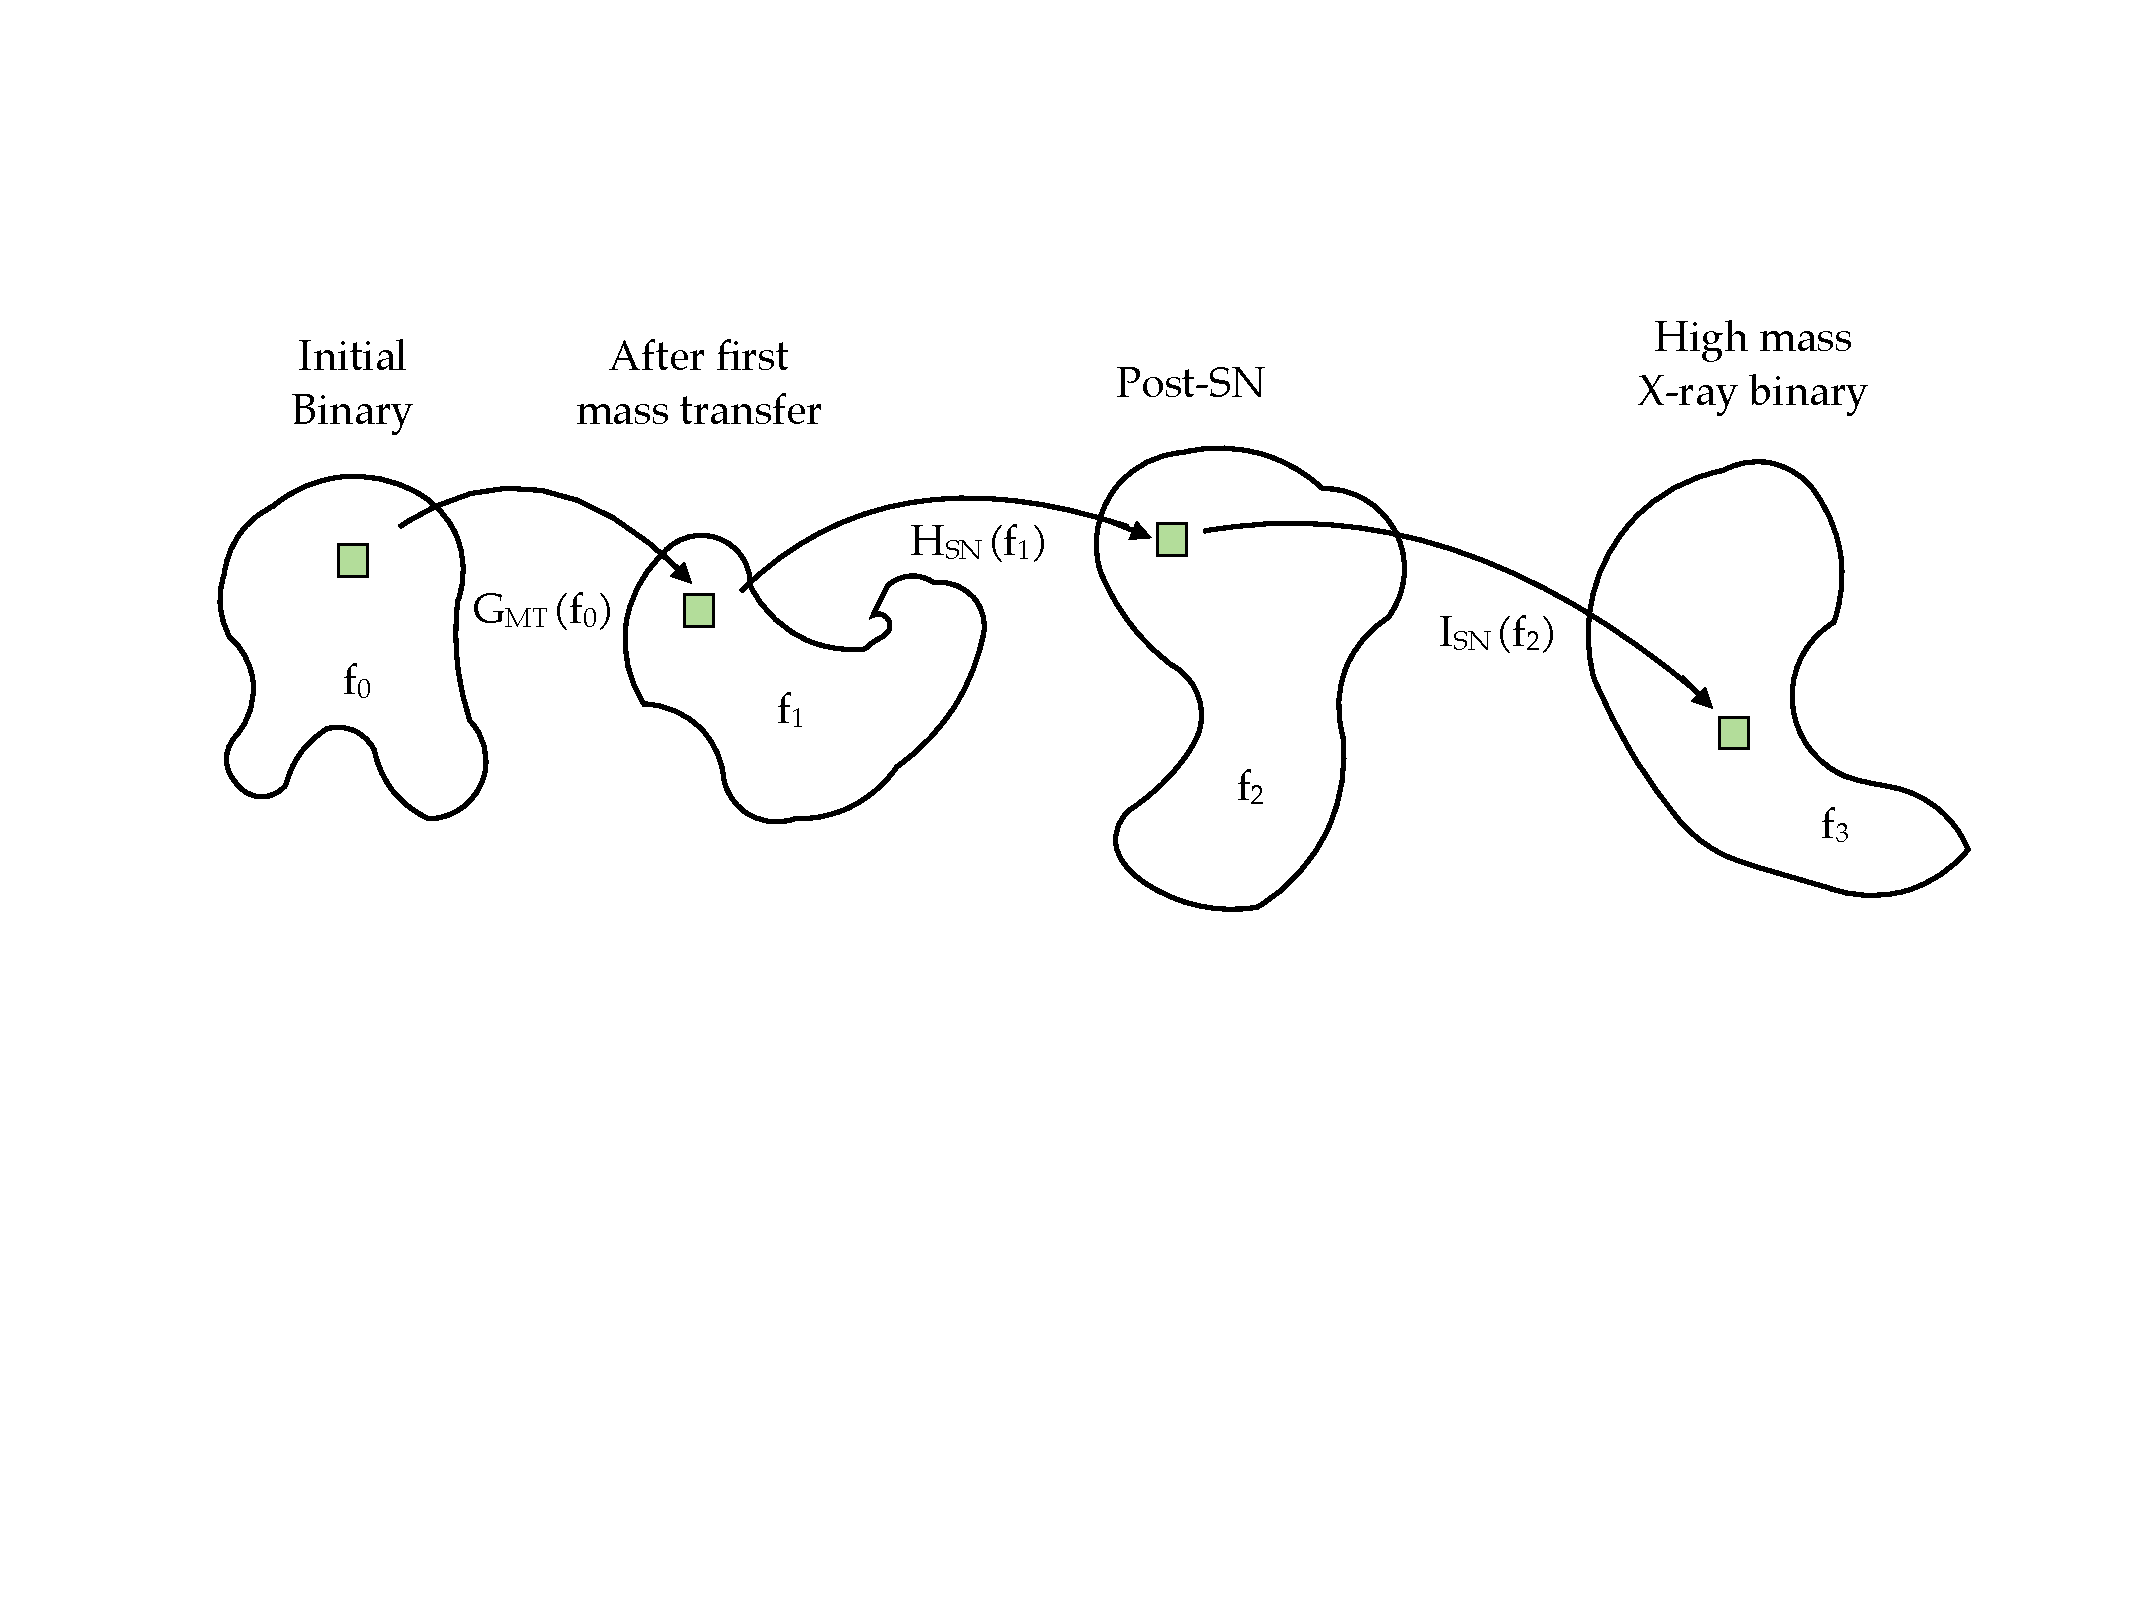
\includegraphics[width=0.95\columnwidth]{Mapping.pdf}
\caption{A mathematical representation of the evolution of a binary from its initial state three separate stages of evolution: the first (stable) mass transfer phase ($G_{\rm MT}$), the primary undergoing core collapse and receiving a natal kick ($H_{\rm SN}$), and the X-ray luminous phase once the second star evolves off the main sequence ($I_{\rm XRB}$). The volume of the three dimensional box around the binary scales with the determinant of the Jacobian matrix for each mapping.}
\label{fig:Mapping}
\end{center}
\end{figure}

Mathematically, these are mappings that can be expressed in a straightforward way:
\begin{eqnarray}
f_1 &=& G_{\rm MT} (f_0) \\
f_2 &=& H_{\rm SN} (f_1) \\
f_3 &=& I_{\rm XRB} (f_2), \\
\end{eqnarray}
which can be combined:
\begin{equation}
f_3 = I_{\rm XRB} \circ H_{\rm SN} \circ G_{\rm MT} ( f_0).
\end{equation}


If we are interesting on an individual system or a small set of binaries, we can opt for a different approach, however.


\begin{comment}
If, however, a reverse mapping exists (or it can be determined numerically), a different approach can be used. This mapping allows one to determine the initial binary state from the observed system:
\begin{equation}
f_0 = G_{\rm MT}^{-1} \circ H_{\rm SN}^{-1} \circ I_{\rm XRB}^{-1} (f_3) .
\end{equation}
Our model provides the probability of the initial state of the binary, $P(f_0)$. The series of transformations from $f_0$ to $f_3$ each shift the volume of phase space around it, affecting the resulting probability. The probability after each transition is determined by scaling the previous probability by the Jacobian of each transition. Determining the probability of the observed binary is now straightforward:
\begin{eqnarray}
P(f_3) &=& P(f_2)  J_{\rm XRB}  \\
  &=& P(f_1)  J_{\rm SN}  J_{\rm XRB}  \\
  &=& P(f_0)  J_{\rm MT}  J_{\rm SN}  J_{\rm XRB} .
\end{eqnarray}
\end{comment}


We choose to adapt and improve upon the Jacobian formalism discussed by Kalogera (1996), Bhadkeamkar \& Ghosh (2012) and others(?). The underlying premise relies upon our ability to map the initial state of a binary through its various stages, until it forms an X-ray luminous object. If this can be done analytically or semi-analytically, such that the first partial derivatives of these mappings can be calculated, then the Jacobians of these mappings can be used to determine how the distribution of binaries evolves without having to randomly generate a population.

If we are interested in determining the probability of any particular binary with some set of observed parameters, such as the set of X-ray binaries in NGC 55, we require both the Jacobians of the three transitions defined above and the reverse mapping. Yet even the most ideal observations of high mass X-ray binaries are unlikely to identify enough parameters to uniquely determine any particular system's prior evolution. To determine the probability of any model producing a binary with observed parameters ($\vec{x}$) we marginalize over latent unobserved parameters ($\vec{y}$):
\begin{equation}
P[f_{\rm obs}(\vec{x})] = \int P[f_3(\vec{x}, \vec{y})] \dd \vec{y}.
\end{equation}
$\vec{y}$ must have enough dimensionality so that the combined $\vec{x}$ and $\vec{y}$ form a complete basis for the binary. This is the basis for the marginalization over $v_k$ and $\theta$ above in Equation \ref{eq:P_marginalized}; $L_x$, $M_2$, and $v_{\rm sys}$ alone do not form a complete basis. In principle, at least, from these five quantities, the initial masses and separation of the binary can be determined.


Below, we discuss each of the three transformations, their reverse mappings, and their Jacobian determinants.


%The reasons for this are many: including complex physics is much easier using Monte Carlo methods, the Jacobian transformation method requires the transformations to be analytic or semi-analytic whereas certain physical processes require numerical integration to accurately calculate, and Monte Carlo methods can easily handle complicated evolutionary channels. 




%Since we are only interested in a small subset of binaries, those that are strong X-ray sources, we can employ the Jacobian transformation method here. The nature of the method is significantly computational cheaper since the region of parameter space explored is, by design, limited to only those binaries we are interested in.



\subsubsection{The First Mass Transfer Phase} \label{sec:trans_MT}

We start with the initial conditions of the binary, which includes three parameters, the primary mass ($M_1$), the secondary mass ($M_2$), and the orbital separation ($A$):
\begin{equation}
\{M_1, M_2, A\} \in f_0.
\end{equation}


Once the first star evolves past its main sequence onto the giant branch, it begins overfilling its Roche lobe. We select only those systems that will undergo stable mass accretion, which can be determined by comparing the thermal time of the secondary with the mass accretion time. This comparison determines whether the transferring matter can lose its entropy fast enough to become incorporated with the companion star, or whether it forms a common envelope. The mapping from the initial binary conditions to the post-mass transfer binary is straightforward. The post mass transfer primary becomes the primary core mass ($M_{1,c}$), while the secondary incorporates the primary's lost envelope. From Ghosh et al.: 
\begin{eqnarray} 
M_1' &=& M_{1,c} \\
M_2' &=& M_2 + f_a (M_1 - M_{1,c}),
\end{eqnarray}
where $f_a$ is a unitless parameter designating the fraction of mass lost by the primary that is accreted by the secondary. The post-mass transfer orbital separation is:
\begin{equation}
A' = A \left[ \frac{M_1 M_2}{M_1' M_2'} \right]^2.
\end{equation}
$M_{1,c}$ can be estimated by:
\begin{equation}
M_{1,c} = M_0 M_1^{1/\xi}, \label{eq:M_He_core}
\end{equation}
where $M_0 = 0.073\ \Msun$ and $\xi = 0.704$. 


The inverse transformation, $G_{\rm MT}$ can be determined from these equations:
\begin{equation}
M_1 = \left( \frac{M_1'}{M_0} \right)^{\xi}, 
\end{equation}
and
\begin{equation}
M_2 = M_2' - \left( \frac{M_1'}{M_0} \right)^{\xi} + M_1'.
\end{equation}
Using these, we can determine $A$ from $A'$:
\begin{equation}
A = \left[ \frac{M_1' M_2'}{M_1 M_2} \right]^2 A'
\end{equation}



Determining the Jacobian matrix of this transformation (which we provide in the appendix) allows us transform the initial binary distribution into the post mass transfer distribution:
\begin{equation}
P(M'_1, M'_2, A') = P(M_1, M_2, A) J_{MT}. \label{eq:P_MT}
\end{equation}
We assume that the binary does not change between the end of the mass transfer phase until the primary undergoes a SN. 




\subsubsection{The Primary's Core Collapse} \label{sec:trans_SN}

We next calculate the post-SN orbital separation ($A''$), systemic velocity ($v_{\rm sys}$), and eccentricity ($e$) based on the equations in Kalogera (1996):
\begin{equation}
A'' = \left[ \frac{2 }{A'}  - \frac{v_1^2}{G(M_{\rm NS} + M_2')} \right]^{-1}. \label{eq:SN_A} \\
%A'' &=& GM_1M_2 \left[ -\left( \frac{M_1''M_2''}{M_1'' + M_2''} \right) v_1^2 + \frac{2GM_1''M_2''}{A'} \right] ^{-1} \label{eq:SN_A} \\
\end{equation}
where $v_1$ is the post-kick velocity of the primary (in the reference frame of an initially stationary secondary):
\begin{equation}
v_1^2 = 2v_k v_r \cos \theta + v_k^2 + v_r^2, \label{eq:v_1}
\end{equation}
where:
\begin{equation}
v_r = \sqrt{\frac{G (M_1' + M_2')}{A'}}. \label{eq:v_r}
\end{equation}
The systemic velocity is:
\begin{equation}
v_{\rm sys}^2 = \beta^2 v_k^2
   + v_r^2 \left( \alpha - \beta \right)^2
   + 2 \beta v_r v_k \cos \theta \left( \alpha - \beta \right)
    \label{eq:SN_v_sys}
\end{equation}
where we have included two substitutions:
\begin{eqnarray}
\alpha &=& \frac{M_1'}{M_1' + M_2'} \\
\beta &=& \frac{M_{\rm NS}}{M_{\rm NS} + M_2'}
\end{eqnarray}


For now, we will ignore eccentricity. However, if the post-SN orbital eccentricity becomes relevant for the evolution of the binary later on, we can include it in the analysis. We include the eccentricity equation below for reference:
\begin{equation}
1-e^2 = \frac{A'^2}{A'' G (M_{\rm NS} + M_2')} \left[ v_k^2 \cos^2\theta + v_k^2 \sin^2 \theta \sin^2 \phi + 2 v_k v_r \cos \theta + v_r^2  \right]. \label{eq:SN_e}
\end{equation}

The reverse mapping of this transformation, $H_{\rm SN}$ is analytic. We first make a substitution:
\begin{eqnarray}
X &=& \frac{\beta - \alpha}{\beta} v_r \nonumber \\
&=& -v_k \cos\theta \pm \sqrt{\frac{v_{\rm sys}^2}{\beta^2} - v_k^2 \sin^2\theta}, \label{eq:SN_X}
\end{eqnarray}
which we obtain by solving Equation \ref{eq:SN_v_sys} for $v_r$. Combining Equations \ref{eq:SN_A}, \ref{eq:v_1}, \ref{eq:v_r}, and \ref{eq:SN_X}, we obtain a quadratic equation for $M_1'$:
\begin{equation}
0 = C_1 M_1'^{2} + C_2 M'_1 + C_3, \label{eq:SN_M_1}
\end{equation}
where the constants, $C_i$, are equal to:
\begin{eqnarray}
C_1 &=& \frac{G(M_{\rm NS} + M'_2)}{A''} + v_k^2 + \frac{M_{\rm NS}^2}{M_2^{'2}}X^2 - 2 v_k \cos \theta \frac{M_{\rm NS}}{M'_2}X \\
C_2 &=& -2M_{\rm NS} \left[ \frac{G(M_{\rm NS} + M'_2)}{A''} + v_k^2 + \frac{M_{\rm NS}^2}{M_2^{'2}}X^2 + \left( 1 - \frac{M_{\rm NS}}{M'_2} \right) v_k \cos \theta X \right] \\
C_3 &=& \frac{G(M_{\rm NS} + M'_2)}{A''} M_{\rm NS}^2 + M_{\rm NS}^2 (v_k^2 + X^2) + 2v_k \cos \theta M_{\rm NS}^2 X - \frac{2(M_{\rm NS} + M'_2)}{M'_2} M_{\rm NS}^2X^2
\end{eqnarray}
Solving Equation \ref{eq:SN_M_1} now provides four separate values for $M_1'$, each of which has a corresponding $A'$ value:
\begin{equation}
A' = G (M_1' + M_2') \left(\frac{M_{\rm NS} - M_1'}{M_1' + M_2'} \right)^2 \left( \frac{M_2'}{M_{\rm NS}} \right)^2 \frac{1}{X^2}. \label{eq:SN_A1}
\end{equation}
Although there are four separate solutions for $M_1'$ and $A'$, three can be removed since we require that $v_r > 0$ and $M'_1 > M_{\rm NS}$. All four must be solved for since it is unknown which of the four solutions is the correct one {\it a priori}.



Derivatives of equations \ref{eq:SN_A} and \ref{eq:SN_v_sys} determine the Jacobian $J_{\rm SN}$. We provide the analytic form for $J_{\rm SN}$ in the Appendix. The probability of the post-SN parameters from the pre-SN parameters and the three kick parameters is:
\begin{equation}
P(M_{\rm NS}, M_2', A'') = P(M_1', M_2', A') J_{\rm SN}. \label{eq:P_SN}
\end{equation}





\subsubsection{The X-ray Luminous Phase} \label{sec:trans_XRB}

Once the secondary evolves onto the core helium burning branch, its luminosity increases, and the star emits a wind accreted by the primary NS. Determining the X-ray luminosity ($L_x$) from the accretion rate ($\dot{M}$) is straightforward: 
\begin{equation}
L = \frac{G M_{\rm NS} \dot{M}}{R_{\rm NS}}.
\end{equation}
We assume a circular binary, the NS accretes from its companion's wind, that the wind is faster than the orbital velocity of the companion, and that the orbital separation, $A$, is significantly greater than the Bondi radius of the NS. Under these assumptions, the fraction of the companion's wind that is accreted by the NS can be determined in a straightforward way:
\begin{equation}
\dot{M} = \left( \frac{G M_{\rm NS}}{V_w^2 A''} \right)^2 \times \dot{M}_{\rm wind}.
\end{equation}
Determining this transformation is difficult; $\dot{M}_{\rm wind}$ is not a simple function of the stellar mass. Typically, stellar models adopt mass loss rates from studies that generate fitting formulae to fundamental stellar parameters for large numbers of stars. Vink et al.\ is the modern standard for high mass stellar winds:
\begin{equation}
\dot{M}_{\rm wind} \propto \frac{L^{2.45} R^{-0.5}}{M^{1.3}}. \label{eq:vink}
\end{equation}
This equation highlights the difficulty. First, $R$ and $L$ must, in general, be determined from stellar evolution codes. Second, the mass loss rates of massive stars are significant, and all three stellar parameters ($R$, $L$, and $M$), and therefore both the mass loss rate and the orbital separation, vary over time. 



There is a subtle but important complication here. From the first mass transfer phase, the secondary gained a significant amount of hydrogen, which, depending on the initial stellar parameters, could more than double its mass. Clearly the stellar lifetimes will be affected. The first mass transfer phase will occur at roughly the helium ignition time for a star of mass $M_1$, $t_{\rm He} (M_1)$. If we assume that stars burn hydrogen at a constant rate throughout their main sequence, the hydrogen mass of the secondary at this point will be:
\begin{equation}
M_{\rm He,2} = \frac{t_{\rm He}(M_1)}{t_{\rm He}(M_2)} M_{\rm He,core}(M_2), \label{eq:M_He}
\end{equation}
where $M_{\rm He,core}(M_2)$ is the helium core mass (at helium ignition) of a star with an initial mass of $M_2$. At this point, the secondary will accrete roughly pure hydrogen from the primary. Since this mass transfer occurs on a thermal timescale, it is effectively instantaneous compared to the stellar lifetime. The rejuvenated secondary star, may have a substantially different mass ($M_2'$), but it is not beginning with a cosmic helium abundance. We can estimate its effective age ($t_{\rm eff}$) by comparing its helium mass from Equation \ref{eq:M_He} with $M_{\rm He,core}(M_2')$, multiplied by the helium ignition time:
\begin{equation}
t_{\rm eff} = \frac{M_{\rm He,2}}{M_{\rm He,core} (M_2') } t_{\rm He} (M_2'). \label{eq:t_eff_1}
\end{equation}
Finally, the total age of the system ($t_b$) is a conditional on our posterior probability. The secondary's effective age at the time of observation, $t_b$, is $t_{\rm eff,obs} = t_{\rm eff} + t_b - t_{\rm He}(M_1)$, which can be expressed using Equations \ref{eq:M_He} and \ref{eq:t_eff_1}:
\begin{equation}
t_{\rm eff,obs} = \frac{M_{\rm He,core}(M_2)}{M_{\rm He,core}(M_2')} \frac{t_{\rm He}(M_1)}{t_{\rm He}(M_2)} t_{\rm He}(M_2')
  + t_b - t_{\rm He}(M_1) \label{eq:t_eff_obs_full}
\end{equation}
Unfortunately, accurately calculating $t_{\rm eff,obs}$ requires both $M_1$ and $M_2$ which can only be determined by evaluating the previous two transformations, discussed in Sections \ref{sec:trans_MT} and \ref{sec:trans_SN}. To get an estimate of how important the transformation is, we first evaluate $t_{\rm eff,obs}$ in the limit of a large initial mass ratio: $M_1 >> M_2$. In this limit, the first term in Equation \ref{eq:t_eff_obs_full} can be ignored:
\begin{equation}
\lim_{M_1 >> M_2}:  t_{\rm eff,obs} \approx t_b - t_{\rm He}(M_2'). \label{eq:t_eff_obs_lim_1}
\end{equation}
We now take the opposite limit, such that $M_1 \approx M_2$. In this limit, $M_1, M_2 \approx M_2'/2$. We can find a similar approximation for $t_{\rm eff,obs}$:
\begin{equation}
\lim_{M_1 \approx M_2}: t_{\rm eff,obs} \approx (2)^{-1/\xi}  t_{\rm He} (M_2') + t_b - t_{\rm He} (M_2'/2).
\end{equation}
While these two approximations will in general differ, the difference between them will provide an estimate of the overall dependence of the stellar merger on the secondary's effective lifetime. Specifically, if the difference between the two limiting $t_{\rm eff,obs}$ is smaller than the uncertainty on the star formation history of the particular region in question, then we can approximate $t_{\rm eff,obs}$ using Equation \ref{eq:t_eff_obs_lim_1}.


The forward mapping, $I_{\rm XRB}$, can be easily achieved in binary evolution codes by evolving the star while integrating the orbital evolution in time. For our problem, we would like to determine the backwards mapping, $I^{-1}_{\rm XRB}$. If we assume the NS only accretes an insignificant portion of the mass during the X-ray luminous phase, the backwards mapping can be found numerically using a two-dimensional root finder. Expressed mathematically, we would like to find $M'_2$ and $A''$ from the observed $L$ and $M''_2$ at a specific time, $t_{\rm obs}$:
\begin{equation}
f_2(M_{\rm NS}, M'_2, A'') = I^{-1}_{\rm XRB} \left[ f_3(M_{\rm NS}, L, M''_2) \right].
\end{equation}
Once $f_2$ is found, the Jacobian determinant, $J_{\rm XRB}$ can be determined numerically, since the forward mapping is known (numerically).

The probability of observing the X-ray binary after time $t_{\rm obs}$, with the observed luminosity is:
\begin{equation}
P(M_{\rm NS}, M''_2, L) = P(M_{\rm NS}, M'_2, A'') J_{\rm XRB}. \label{eq:P_XRB}
\end{equation}



\subsection{P($t_b \given C)$}

The final term gives the probability of a birth time for a particular cluster. The birth time probability is directly related to the star formation rate at that time:
\begin{equation}
P(t_b \given C) \propto {\rm SFR}(t_b).
\end{equation} 
Determining this term therefore requires a knowledge of the star formation history of each star forming cluster. Multi wavelength observations have allowed approximate knowledge of the star formation histories for most of the star forming regions in NGC 55, at least within the recent past.

\subsection{P($P(\vec{m} \given M_2, M)$)}

Finally, we need to determine the probability of observing the set of optical observations for each object $\vec{m}$ given a companion mass $M_2$. Since the distance to NGC 55 is known, and we have {\it HST} photometry for most of the X-ray binaries, this probability should be known quite accurately:
\begin{equation}
P(\vec{m} \given M_2, M) \approx \delta\left[ \vec{m} - f(M_2) \right],
\end{equation}
where $f(M_2)$ is some function of the companion mass determined from stellar evolution models. We use both the models from the Geneva group and the Padova group here. However, for certain masses, magnitudes do not vary strongly as a function of mass, and we must perform the integral over $M_2$ in Equation \ref{eq:marginalized}.

 



\subsection{Prior Probabilities}

As part of our model, we standard distributions for the initial parameters of the binary, that the initial primary mass follows a power law, the mass ratio follows a uniform distribution, and the binary separation follow a log uniform distribution:
\begin{eqnarray}
P(M_1) &\propto& M^{\alpha} \\
P(q) &\propto& 1 \\
P(A) &\propto& A^{-1}.
\end{eqnarray}
These combine into the probability of our initial binary:
\begin{equation}
P(M_1, q, A) = \frac{M^{\alpha}}{A}. \label{eq:P_init}
\end{equation}
In our model, we assume the NS natal kick follows a single Maxwellian distribution:
\begin{equation}
P(v_k \given M) = \sqrt{\frac{2}{\pi}} \frac{v_k^2} {\sigma^3} {\rm exp} \left[ -v_k^2 / 2 \sigma^2 \right]. \label{eq:P_v_k}
\end{equation}
Since the kick distribution is isotropic, $P(\theta)$ is:
\begin{equation}
P(\theta) = \sin \theta. \label{eq:P_theta}
\end{equation}
{\bf What other model parameters do we have here?}

The combined probability we are looking for, $P(L_x, M_2, v_{\rm sys} \given t_b, M)$ can now be determined from combining Equations \ref{eq:P_marginalized}, \ref{eq:P_MT}, \ref{eq:P_SN}, \ref{eq:P_XRB}, \ref{eq:P_init}, \ref{eq:P_v_k}, and \ref{eq:P_theta}.



\subsection{Numerical Method}

We use DFM's {\tt emcee}.



\section{Test Cases}

... Make a test model to check our code and see if it actually works.

\section{Results}

... Apply our model to the data from NGC 55. 

\section{Discussion}

... First stab at a difficult problem. This is the basics, but generalization to X-ray populations in all galaxies should be possible.

... What does this imply about our understanding of NGC 55? What about binary population synthesis? Kick velocities? High mass binary evolution?



\appendix

\section{Jacobians for Transformations}

We provide the Jacobian for $G_{\rm MT}$ below:
\[  J_{\rm MT} = \left( \begin{array}{ccc}
\frac{\partial M_1'}{\partial M_1} & \frac{\partial M_1'}{\partial M_2} & \frac{\partial M_1'}{\partial A}  \\[0.3em]
\frac{\partial M_2'}{\partial M_1}  & \frac{\partial M_2'}{\partial M_2} & \frac{\partial M_2'}{\partial A} \\[0.3em]
\frac{\partial A'}{\partial M_1} & \frac{\partial A'}{\partial M_2} & \frac{\partial A'}{\partial A}  \end{array} \right)\]

{\bf These need to be worked out}


\begin{comment}
The partial derivatives are:
\begin{eqnarray}
\frac{\partial M_1'}{\partial M_1} &=& \frac{M_0}{\xi} M_1^{(1 - \xi)/ \xi} \\
\frac{\partial M_1'}{\partial M_2} &=& 0 \\
\frac{\partial M_1'}{\partial A} &=& 0 \\
\frac{\partial M_2'}{\partial M_1} &=& 1 + \frac{M_0}{\xi} M_1^{(1 - \xi)/ \xi} \\
\frac{\partial M_2'}{\partial M_2} &=& 1 \\
\frac{\partial M_2'}{\partial A} &=& 0 \\
\frac{\partial A'}{\partial M_1} &=& A \frac{M_2^2}{M_0^2} M_1^{2 (\xi - 1)/\xi} 
     \left( M_1 + M_2 + M_0 M_1^{1/\xi} \right)^2
     \left[ \frac{2 - 2/\xi}{M_1} + \frac{1 - \frac{M_0}{\xi}M_1^{(1-\xi)/\xi}}{M_1 + M_2 + M_0 M_1^{1/\xi}} \right] \\
\frac{\partial A'}{\partial M_2} &=& \frac{2 A M_1^2 M_2^2}{M_0^2 M_1^{1/\xi}} 
     \left( M_1 + M_2 - M_0 M_1^{1/\xi} \right)
     \left( \frac{M_1 + M_2 - M_0 M_1^{1/\xi}}{M_2} + 1 \right) \\
\frac{\partial A'}{\partial A} &=& \frac{M_2^2 M_1^2}{M_0^2 M_1^{2/\xi}} \left( M_1 + M_2 + M_0 M_1^{1/\xi} \right)^2.
\end{eqnarray}
Here, $M_0 = 0.073\ \Msun$ and $\xi = 0.704\ \Msun$, as defined in the text above.

The Jacobian for $H_{\rm SN}$ is below:
\[  J_{\rm MT} = \left( \begin{array}{ccc}
\frac{\partial v_{\rm sys}}{\partial M_1'} & \frac{\partial v_{\rm sys}}{\partial M_2'} & \frac{\partial v_{\rm sys}}{\partial A'}  \\[0.3em]
\frac{\partial M_2''}{\partial M_1'}  & \frac{\partial M_2''}{\partial M_2'} & \frac{\partial M_2''}{\partial A'} \\[0.3em]
\frac{\partial A''}{\partial M_1'} & \frac{\partial A''}{\partial M_2'} & \frac{\partial A''}{\partial A'}  \end{array} \right)\]
The partial derivatives are:
\begin{eqnarray}
\frac{\partial v_{\rm sys}}{\partial M_1'} &=& \frac{1}{2} \frac{M_1''}{(M_1''+M_2'')(M_1'+M_2')} 
     \frac{v_r^2 + v_k v_r \cos \theta}{\sqrt{2 v_k v_r \cos \theta + v_k^2 + v_r^2}} \\
\frac{\partial v_{\rm sys}}{\partial M_2'} &=& 0 \\    
\frac{\partial v_{\rm sys}}{\partial A'} &=& -\frac{1}{2A'} \frac{M_1''}{M_1'' + M_2''} 
     \frac{v_k v_r \cos \theta + v_r^2 }{\sqrt{2 v_k v_r \cos \theta + v_k^2 + v_r^2}} \\
\frac{\partial M_2''}{\partial M_1'} &=& 0 \\
\frac{\partial M_2''}{\partial M_2'} &=& 0 \\
\frac{\partial M_2''}{\partial A'} &=& 0 \\
\frac{\partial A'''}{\partial M_1'} &=& 
\end{eqnarray}
\end{comment}

\acknowledgements
Acknowledgements:
It is a pleasure to thank...
Funding...
Code...

\end{document}
